\section{Natural logarithm}

Natural logarith (denoted as \texttt{ln} on handheld calculators, and sometimes denoted just as \texttt{log})
is logarithm of base $e=2.718281828...$.
Where this constant came from?

\subsection{Savings account in your bank}

Let's say you make a deposit into bank, say, 100 dollars (or any other currency).
They offer 2.5\% per year (annual percentage yield).
This mean, you'll can get doubled amount of money (200 dollars) after 40 years.
So far so good.
But some banks offers compound interest.
Also called ``complex percent'' in Russian language, where ``complex'' in this phrase is closer to the word ``folded''.
This mean, after each year, they pretend you withdraw your money with interest, then redeposit them instantly.
Banks also say that the interest is recapitalized once a year.
Let's calculate final amount of money after 40 years:

\lstinputlisting[caption=Python code]{log/APY1.py}

\begin{lstlisting}
year= 0 amount at the end 102.5
year= 1 amount at the end 105.0625
year= 2 amount at the end 107.6890625
year= 3 amount at the end 110.381289063
...
year= 36 amount at the end 249.334869861
year= 37 amount at the end 255.568241608
year= 38 amount at the end 261.957447648
year= 39 amount at the end 268.506383839
\end{lstlisting}

The thing is that the final amount (268.50...) is aimed toward $e$ constant.

Now there is another bank, which offers to recapitalize your deposit each month.
We'll rewrite our script slightly:

\lstinputlisting[caption=Python code]{log/APY2.py}

\begin{lstlisting}
year= 0 month= 0 amount 100.208333333
year= 0 month= 1 amount 100.417100694
year= 0 month= 2 amount 100.626302988
year= 0 month= 3 amount 100.835941119
...
year= 39 month= 8 amount 269.855455383
year= 39 month= 9 amount 270.417654248
year= 39 month= 10 amount 270.981024361
year= 39 month= 11 amount 271.545568162
\end{lstlisting}

The final result is even closer to $e$ constant.

Let's imagine there is a bank which allows to recapitalize each day:

\lstinputlisting[caption=Python code]{log/APY3.py}

\begin{lstlisting}
year= 0 month= 0 day= 0 amount 100.006944444
year= 0 month= 0 day= 1 amount 100.013889371
year= 0 month= 0 day= 2 amount 100.02083478
year= 0 month= 0 day= 3 amount 100.027780671
...
year= 39 month= 11 day= 26 amount 271.762123927
year= 39 month= 11 day= 27 amount 271.780996297
year= 39 month= 11 day= 28 amount 271.799869977
year= 39 month= 11 day= 29 amount 271.818744968
\end{lstlisting}

The final amount of money is more closer to $e$ constant.

If to imagine some really crazy bank client who redeposit his deposit infinite number of times per each day, the final value after 40 years
would be $100 \cdot e$.
It's not possible in the real world, so the final amount is approaches this value, but is never equal to it.
Mathematically speaking, its limit is $100 \cdot e$.

\subsection{Exponential decay}

\subsubsection{Capacitor discharge}

% TODO redraw! ибо спизжено. https://en.wikipedia.org/wiki/Talk%3ARC_circuit#RC_Circuits
\begin{figure}[H]
\centering
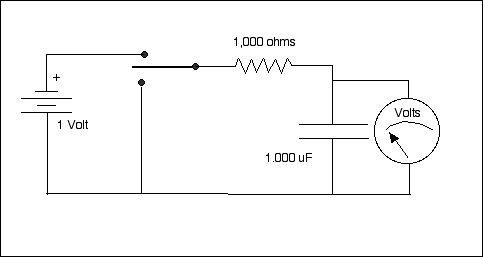
\includegraphics[scale=0.66]{log/Schematic_of_Battery_and_Capacitor.jpg}
\end{figure}

From electronics engineering course we may know that the capacitor discharging by half after $RC\ln(2)$ seconds,
where C is capacity of capacitor in farads and R resistance of resistor in ohms.
Given $1k\Omega$ resistor and $1000 \mu F$ capacitor, what its voltage after 1 seconds will be? after 2 seconds?
It's discharge can be calculated using this equation:

\LARGE\[
V=V_0 \cdot e^{\frac{-t}{RC}}
\]
\normalsize

\dots where $V_0$ is initial charge in volts, $t$ is time in seconds and $e$ is base of natural logarithm.

Let's see it in Wolfram Mathematica:

\begin{lstlisting}[caption=Wolfram Mathematica]
r = 1000; (* resistance in ohms *)

c = 0.001; (* capacity in farads *)

v = 1; (* initial voltage *)

Plot[v*E^((-t)/(r*c)), {t, 0, 5}, 
 GridLines -> {{Log[2], Log[2]*2, Log[2]*3}, {0.5, 0.25, 0.125}},
 Epilog -> {Text["ln(2)", {Log[2], 0.05}], 
   Text["ln(2)*2", {Log[2]*2, 0.05}], 
   Text["ln(2)*3", {Log[2]*3, 0.05}],
   Text["1/2", {0.1, 0.5}], Text["1/4", {0.1, 0.25}], 
   Text["1/8", {0.1, 0.128}]}, AxesLabel -> {seconds, voltage}]
\end{lstlisting}

\begin{figure}[H]
\centering
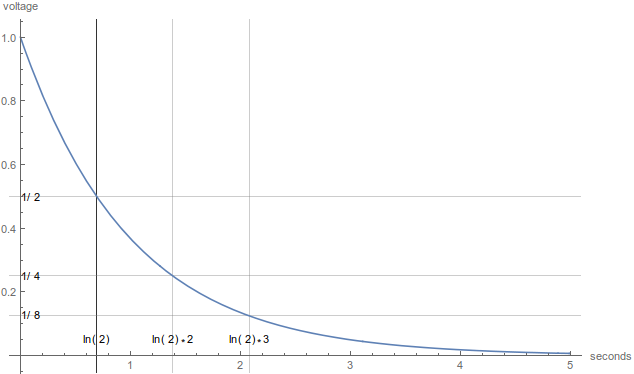
\includegraphics[scale=0.66]{log/capacitor_discharge.png}
\caption{Capacitor voltage during discharge}
\end{figure}

As we can see, $\frac{1}{2}$ of initial charge is left after $ln(2)$ seconds (~0.69...), 
and $\frac{1}{4}$ of charge is left after $ln(4)$ seconds (~1.38...).

Indeed, if we interesting in precise time in seconds, when charge will be $\frac{1}{x}$, just calculate $ln(x)$.

Now here is the same plot, but I added two more labels, $\frac{1}{3}$ and $\frac{1}{7}$:

\begin{lstlisting}[caption=Wolfram Mathematica]
Plot[v*E^((-t)/(r*c)), {t, 0, 5}, 
 GridLines -> {{Log[3], Log[7]}, {1/3, 1/7}},
 Epilog -> {Text["ln(3)", {Log[3], 0.05}], 
   Text["ln(7)", {Log[7], 0.05}],
   Text["1/3", {0.1, 1/3}], Text["1/7", {0.1, 1/7}]}, 
 AxesLabel -> {seconds, voltage}]
\end{lstlisting}

\begin{figure}[H]
\centering
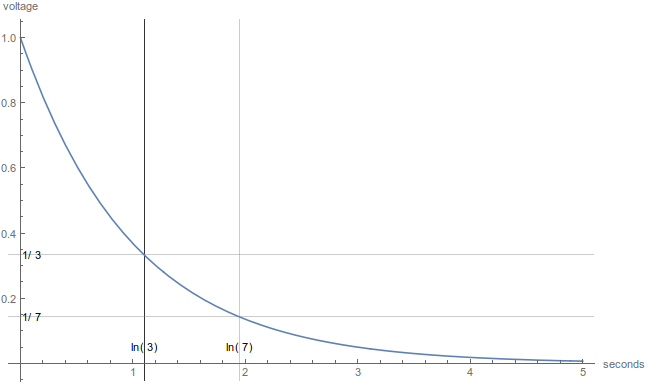
\includegraphics[scale=0.66]{log/capacitor_discharge2.png}
\caption{Capacitor voltage during discharge}
\end{figure}

\dots and we see that these points corresponds to $ln(3)$ and $ln(7)$.
That means, $\frac{1}{3}$ of charge is left after $ln(3) \approx 1.098...$ seconds and $\frac{1}{7}$ of charge after $ln(7) \approx 1.945...$ seconds.

\subsubsection{Radioactive decay}

Radioactive decay is also exponential decay.
Let's take Polonium 210 as an example\footnote{\url{https://en.wikipedia.org/wiki/Polonium}}.
It's half-life (calculated) is $\approx 138.376$ days.
That means that if you've got 1kg of Polonium 210, after $\approx 138$ days, half of it (0.5 kg) left as \textsuperscript{210}Po and 
another half is transformed into \textsuperscript{206}Pb (isotope of lead\footnote{\url{https://en.wikipedia.org/wiki/Isotopes_of_lead\#Lead-206}}).
After another $\approx 138$ days, you'll get $\frac{3}{4}$ of isotope of lead and $\frac{1}{4}$ will left as \textsuperscript{210}Po.
After another $\approx 138$ days, amount of Polonium will be halved yet another time, etc.

The equation of radioactive decay is:

\[
N=N_{0}e^{-\lambda t}
\]

\dots where $N$ is number of atoms at some point of time, $N_{0}$ is initial number of atoms, $t$ is time, $\lambda$ is decay constant.
Decay of Polonium is exponential, but decay constant is the constant, defining how fast (or slow) it will fall.

Here we go in Mathematica, let's get a plot for 1000 days:

\begin{lstlisting}[caption=Wolfram Mathematica]
l = 0.005009157516910051; (* decay constant of Polonium 210 *)

hl = Log[2]/l
138.376

Plot[E^(-l*t), {t, 0, 1000}, 
 GridLines -> {{hl, hl*2, hl*3}, {0.5, 0.25, 0.125}}, 
 Epilog -> {Text["hl", {hl, 0.05}], Text["hl*2", {hl*2, 0.05}], 
   Text["hl*3", {hl*3, 0.05}], Text["1/2", {30, 0.5}], 
   Text["1/4", {30, 0.25}], Text["1/8", {30, 0.128}]}, 
 AxesLabel -> {days, atoms}]
\end{lstlisting}

\begin{figure}[H]
\centering
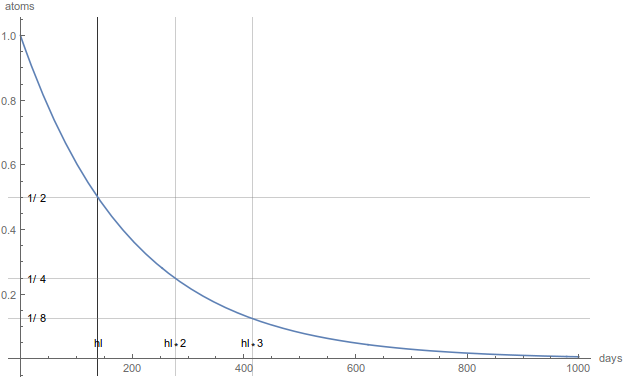
\includegraphics[scale=0.66]{log/210po.png}
\caption{Exponential decay of Polonium 210}
\end{figure}

\subsubsection{Beer froth}

There is even the paper (got Ig Nobel prize in 2002), author's of which demonstrates that beer froth is also decays exponentially:
\url{http://iopscience.iop.org/0143-0807/23/1/304/},
\url{https://classes.soe.ucsc.edu/math011a/Winter07/lecturenotes/beerdecay.pdf}.

\begin{figure}[H]
\centering
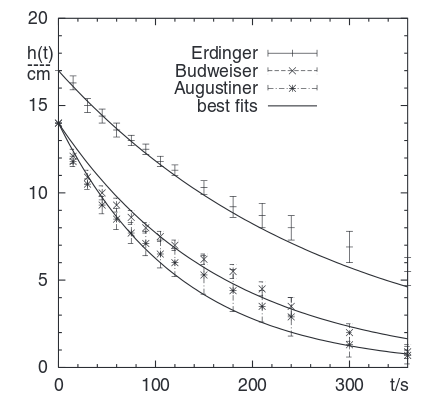
\includegraphics[scale=0.66]{log/beer.png}
\caption{Results from the paper}
\end{figure}

The paper can be taken as a joke, nevertheless, it's a good demonstration of exponential decay.

\subsubsection{Conclusion}

Capacitor discharge and radioactive decay obeys the same law of halving some amount after equal gaps of time:

\[
amount=amount_{0} \cdot e^{- decay\_constant \cdot time}
\]

Decay constant in case of capacitor discharge defined by product of resistance and capacity.
The bigger one of them, the slower decay.

Natural logarithm is used to calculate gap of time (half-life or half-time) judging by decay constant.

